\documentclass[a4paper, 10pt]{article}
\usepackage[utf8]{inputenc}
\usepackage[english,russian]{babel}
\usepackage{fancyhdr}
\usepackage{caption}
\usepackage[left=1.5cm,right=1.5cm,top=2cm,bottom=1.5cm,bindingoffset=0cm]{geometry}
\captionsetup{labelsep=period}
\pagestyle{fancy}
\usepackage{listings,longtable,amsmath,amsfonts,graphicx,tikz,tabularx}

\lstset{
    basicstyle=\footnotesize,
    breakatwhitespace=false,
    breaklines=true,
    extendedchars=true,
    keepspaces=true,
    keywordstyle=\bfseries,
    numbers=left,
    numbersep=3pt,
    numberstyle=\tiny,
    showspaces=false,
    showstringspaces=false,
    showtabs=false,
    stepnumber=1,
    stringstyle=\emph,
    tabsize=2
}
\usepackage[export]{adjustbox}
\usepackage{graphicx}
\graphicspath{ {images/} }

\renewcommand{\headrulewidth}{0pt}
\fancyfoot[L] {\thepage\bf}
\fancyfoot[C] {}

\begin{document}
    \begin{titlepage}
        \begin{center}
            \large
            Университет ИТМО
            \vspace{3cm}


            Кафедра вычислительной техники
            \vspace{4cm}

            \textsc{ \textbf{Отчёт по лабораторной работе  № 1} \\ по дисциплине: "Схемотехника ЭВМ"}\\Вариант №5\\[8mm]

            \bigskip
        \end{center}
        \vspace{3cm}

        \hfill\begin{flushright}
             Студенты: \\
             \vfill
             Преподаватель: \\
        \end{flushright}
        \vfill
        \vfill
        \vfill
        \vfill
        \vfill
        \begin{center}
            Санкт-Петербург \\2016 г.
        \end{center}
    \end{titlepage}
   \newpage
    \section*{Содержание}
        \begin{enumerate}
            \item Цели работы.
            \item RTL модель.
            \item Тест-бенч.
            \item Временные диаграммы.
            \item Листинг.
            \item Вывод.
        \end{enumerate}

    \section*{Цели работы}

        \begin{enumerate}
            \item Знакомство с основами проектирования цифровых устройств с использованием языка структурно-функционального описания аппаратуры Verilog HDL.
            \item Освоение работы с базовыми дискретными элементами ввода/вывода: светодиоды, позиционные переключатели, семисегментные индикаторы. 
            \item  Знакомство с маршрутом проектирования цифровых схем для ПЛИС. 
        \end{enumerate} 
     \section*{RTL модель}
        \begin{figure}[h!]
            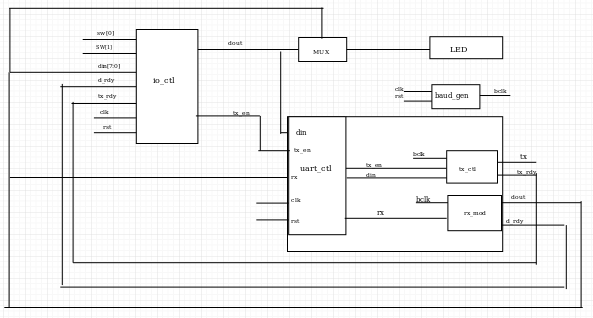
\includegraphics[scale=0.7]{../images/rtl.png}
        \end{figure}
     \section*{Тест-бенч}
        \lstinputlisting[language=Verilog]{../test_bench/test_animation.v}
        \lstinputlisting[language=Verilog]{../test_bench/test_time_mode.v}
        \lstinputlisting[language=Verilog]{../test_bench/test_sw_mode.v}
     \section*{Временные диаграммы}
        \begin{figure}[h!]
            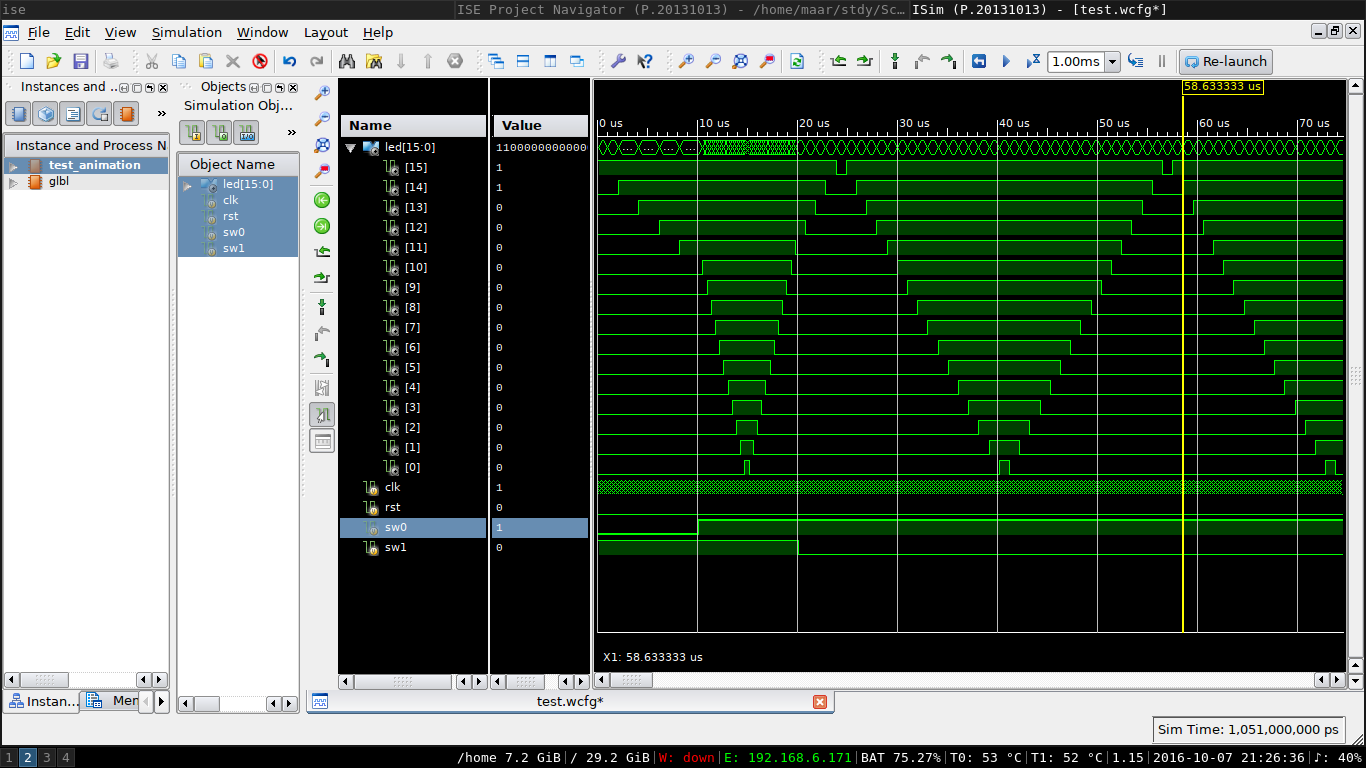
\includegraphics[scale=0.7]{../images/animation.png}
        \end{figure}
        \begin{figure}[h!]
            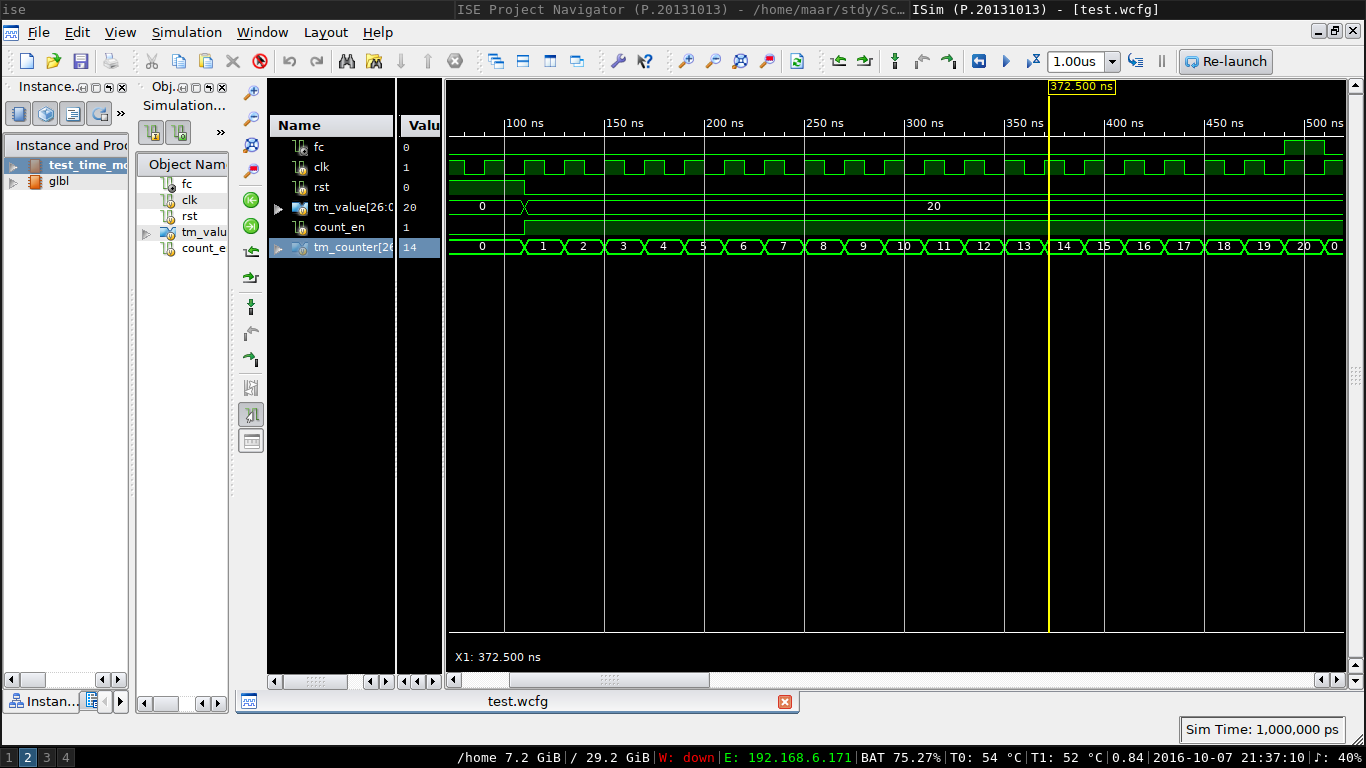
\includegraphics[scale=0.7]{../images/time_mode.png}
        \end{figure}
        \begin{figure}[h!]
            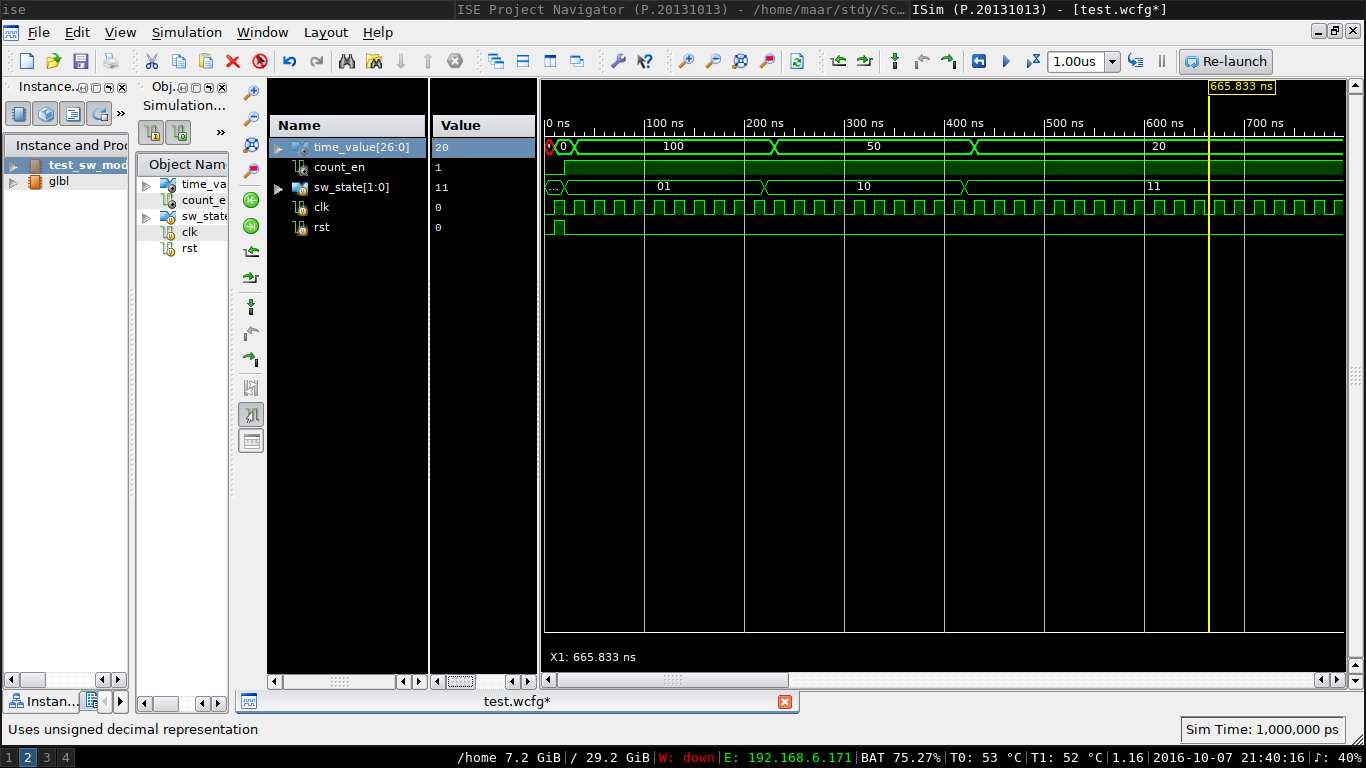
\includegraphics[scale=0.7]{../images/sw_mode.png}
        \end{figure}
        Описание сигналов:
        \begin{itemize}
            \item clk/rst -- сигналы тактового генератора и сброс соответственно;
            \item sw0/sw1 -- входные сигналы с переключателей, определяющие скоростной режим;
            \item led[15:0] -- выходные сигналы на LED'ы, отображающих анимацию;
            \item count\_en -- сигнал, разрешающий счёт ( необходим для запрета счёта в состоянии STOP);
            \item tm\_value -- текущее время, определяемое состоянием sw0/sw1;
            \item tm\_counter -- счётчик времени;
            \item fc -- сигнал для счётчик кадров;
            \item fm\_no -- номер текущего кадра;
            \item counter -- счётчик кадров.
        \end{itemize}

     \section*{Листинг}
        \lstinputlisting[language=Verilog]{../src/switches.v}
        \lstinputlisting[language=Verilog]{../src/sw_mode.v}
        \lstinputlisting[language=Verilog]{../src/time_mode.v}
        \lstinputlisting[language=Verilog]{../src/frame_counter.v}
        \lstinputlisting[language=Verilog]{../src/next_frame.v}
        \lstinputlisting[language=Verilog]{../src/animation.v}

    \section*{Вывод}

\end{document}
